\documentclass[12pt]{article}
\usepackage[utf8]{inputenc} % default from sharelatex
\usepackage[a4paper, left=30mm, right=30mm, top=30mm, bottom=30mm]{geometry}
% dont break my code
\usepackage{indentfirst} % to indent fist paragraph
\usepackage[brazilian]{babel} % BR
\usepackage{listings} % to show code
\usepackage{xcolor} % to colors
\usepackage{hyperref} % to links
\usepackage{graphicx} % to have pictures

\graphicspath{{images/}}

\lstset{
  language=Python,
  basicstyle=\ttfamily\small,
  numberstyle=\footnotesize,
  numbers=left,
  backgroundcolor=\color{gray!10},
  frame=single,
  tabsize=2,
  rulecolor=\color{black!30},
  title=\lstname,
  escapeinside={\%*}{*)},
  breaklines=true,
  breakatwhitespace=true,
  framextopmargin=2pt,
  framexbottommargin=2pt,
  extendedchars=false,
  inputencoding=utf8,
  commentstyle=\color{blue},
  keywordstyle=\color{purple},
  showstringspaces=false,
  stringstyle=\color{red}
}

\hypersetup{
  colorlinks=true,
  urlcolor=blue
}

\title{
  Geradores de números pseudo-aleatórios: \\
  \large Inversive congruential, Lagged Fibonacci e Linear congruential}

\author{Lucas João Martins}
\date{}

\begin{document}

\maketitle

\section{Códigos das implementações}
\lstinputlisting{icg.py}
\lstinputlisting{lfg.py}
\lstinputlisting{lcg.py}

\section{Explicação dos algoritmos}
O inversive congruential generator, também conhecido como ICG, foi desenvolvido
por Eichenauer e Lehn em 1986 e trata-se de um gerador de números
pseudo-aleatórios que é baseado em recursão não linear. A sua congruência é
definida por:
\begin{equation}
  x_{i+1} \equiv ax_i^{-1} + c \ \ (mod \ \ q)
\end{equation}

Onde $x_i^{-1}$ é a função modular inversa entre $x$ e $q$. Os outros
componentes dessa relação já foram explicados na documentação do código.
Importante citar que para um correto funcionamento da relação $x$ e $q$ precisam
ser coprimos, e, que essa verificação não é realizada no código implementado. O
máximo período que o ICG pode alcançar é de $q$ unidades.

O lagged fibonacci generator, também conhecido como LFG, é um gerador de números
pseudo-aleatórios que é baseado em uma generalização da sequência de Fibonacci.
A sua concruência é definida por:
\begin{equation}
  p_{n} \equiv p_{n-j} \star p_{n-k} \ \ (mod \ \ m)
\end{equation}

Onde $\star$ denota uma operação binária qualquer, ou seja, pode ser adição,
subtração, multiplicação ou um xor. Os outros atributos dessa relação já foram
explicados na documentação do código. A implementação do gerador nesse trabalho
faz uso do additive lagged fibonacci generator, também chamado de ALFG, ou seja,
a operação binária escolhida foi a adição. O máximo período que o ALFG pode
alcançar é de $(2^k - 1)2^{p-1}$ unidades.

O linear congruential generator, também conhecido como LCG, foi desenvolvido por
D. H. Lehmer em 1948 e trata-se de um popular gerador de números
pseudo-aleatórios que é baseado em uma equação linear. A sua relação de
recorrência é definida por:
\begin{equation}
  X_{n+1} = (aX_n + c) \ \ mod \ \ m
\end{equation}

Os atributos apresentados já foram explicados na documentação do código. O
máximo período que o LCG pode alcançar é de $m$ unidades

Todos os três geradores possuem regras associadas as suas variáveis e também as
suas formas de operações que podem ser classificadas, de maneira informal, em
dois tipos:
\begin{enumerate}
  \item Essenciais para o funcionamento do gerador;
  \item Responsáveis por maximizar o desempenho do gerador.
\end{enumerate}

Optou-se por não implementar regras do segundo tipo, mas mais informações sobre
elas podem ser obtidas nas referências citadas. Já com relação às regras do
primeiro tipo, experimentou-se utilizar três estratégias diferentes:
\begin{itemize}
  \item Não permitir a instanciação do gerador, o que foi feito no LCG;
  \item Não fazer nada em nível de código e esperar que quem o utilize saiba das
  regras, aplicado no ICG;
  \item Permitir a instanciação do gerador, mas não permitir a geração dos
  números, utilizado no LFG.
\end{itemize}

\section{Comparação entre os algoritmos}
\begin{table}[h]
  \centering
  \caption{5 números pseudo-aleatórios grandes}
  \begin{tabular}{|c|c|c|}
  \hline
  Gerador & Tamanho do número em bits & Tempo gasto  \\ \hline
  ICG     & 27 & 1m15,687s \\ \hline
  ICG     & mais que 30 & Muito tempo, impraticável \\ \hline
  LCG     & 40 & 0m0,023s  \\ \hline
  LFG     & 40 & 0m0,037s  \\ \hline
  LCG     & 56 & 0m0,027s  \\ \hline
  LFG     & 56 & 0m0,043s  \\ \hline
  LCG     & 80 & 0m0,030s  \\ \hline
  LFG     & 80 & 0m0,035s  \\ \hline
  LCG     & 128 & 0m0,023s  \\ \hline
  LFG     & 128 & 0m0,033s  \\ \hline
  LCG     & 168 & 0m0,027s  \\ \hline
  LFG     & 168 & 0m0,040s  \\ \hline
  LCG     & 512 & 0m0,027s  \\ \hline
  LFG     & 512 & 0m0,043s  \\ \hline
  LCG     & 2048 & 0m0,023s  \\ \hline
  LFG     & 2048 & Overflow \\ \hline
  LCG     & 4096 & 0m0,023s  \\ \hline
  \end{tabular}
\end{table}

Ao comparar o LCG com o ICG, percebe-se o seguinte:
\begin{itemize}
  \item O ICG é a versão não linear do LCG;
  \item O LCG apresenta diversas regularidades não desejadas devido a sua
  linearidade;
  \item O resultado do LCG é reticulado, enquanto que o do ICG não é,
\end{itemize}

Já ao comparar o LFG contra o LCG e o ICG, pode-se destacar:
\begin{itemize}
  \item O LFG requer que $k$ unidades sejam armazenadas para poder gerar um
  único número, enquanto que os outros dois só necessitam do armazenamento de
  uma unidade
  \item O período máximo do LCG e do ICG é limitado ao valor do seu módulo,
  enquanto que o LFG não é, e, por isso pode atingir um valor bem maior do que o
  dos outros dois já citados
\end{itemize}

\section{Complexidade dos algoritmos}
\begin{itemize}
  \item Inversive congruential generator: $O(n * q)$
  \begin{itemize}
    \item Devido aos laços nas linhas 44 e 74 do código.
  \end{itemize}
  \item Lagged Fibonacci generator: $O(n * k)$
  \begin{itemize}
    \item Devido aos laços nas linhas 94 e 95 do código.
  \end{itemize}
  \item Linear congruential generator: $O(n)$
    \begin{itemize}
      \item Devido ao laço na linha 51 do código.
    \end{itemize}
\end{itemize}

\section{Os números são aleatórios?}
\begin{figure}[h]
  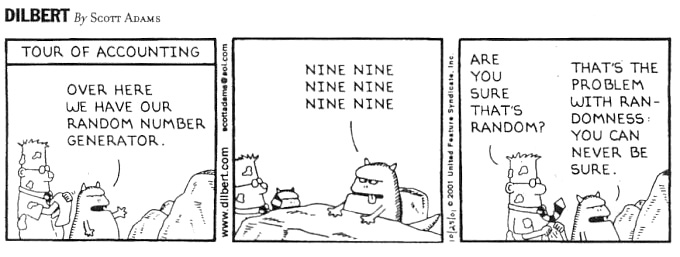
\includegraphics[width=\linewidth]{dilbert}
\end{figure}

Uma resposta curta: você não consegue afirmar se algo é aleatório ou não,
conforme Dilbert já falou um dia.

Uma resposta longa: há diferentes maneiras de interpretar o significado da
aleatoriedade, pois isso pode ser feito do ponto de vista estatístico, ou do
ponto de vista da complexidade de Kolmogorov, ou até mesmo do ponto de vista
criptográfico. Entretanto, nenhum desses pontos de vista conseguem afirmar se
algo é aleatório ou não.

Uma possível solução: se o ponto de vista estatístico for o escolhido, então há
diversos testes que podem mensurar a qualidade de números aleatórios. Testes de
Diehard, desenvolvido em 1995 por George Marsaglia, e os testes de Charmaine
Kenny, desenvolido em 2005, são alguns exemplos de conhecidas baterias de testes
que realizam essa verificação de qualidade.

\section{Referências}
Inversive congruential generator:
\begin{itemize}
  \item \href{https://en.wikipedia.org/wiki/Inversive_congruential_generator}
    {Wikipedia}
  \item
    \href
    {https://www.khanacademy.org/computing/computer-science/cryptography/modarit
    hmetic/a/modular-inverses}{Khan
    Academy}
  \item
    \href{https://books.google.com.br/books?id=OjUyDwAAQBAJ&printsec=frontcover#v=onepage&q&f=false}
    {The Mathematical-Function Computation Handbook}, Nelson H.F. Beebe
  \item \href{http://random.mat.sbg.ac.at/generators/wsc95/inversive/node2.html}
    {pLab}
  \item \href{http://www.sciencedirect.com/science/article/pii/0377042792901909}
    {Construction of inversive congruential pseudorandom number generators with
    maximal period length}, Jürgen Eichenauer-Herrmann, 2002
  \item \href{http://www.cs.fsu.edu/~mascagni/papers/RICP2000_2.pdf}
    {Parallel inversive congruential generators: Software and
    field-programmable gate array implementations}, Michael Mascagni e Shahram
    Rahimi, 2001
\end{itemize}

Lagged Fibonacci generator:
\begin{itemize}
  \item
    \href{http://astro.uchicago.edu/~andrey/classes/rseminar/docs/aluru.pdf}
    {Lagged Fibonacci Random Number Generators for Distributed Memory Parallel
    Computers}, Srinivas Aluru, 1997
  \item \href{https://pthree.org/2015/05/29/the-lagged-fibonacci-generator/}
    {Aaron Toponce}
  \item \href{https://en.wikipedia.org/wiki/Lagged_Fibonacci_generator}
    {Wikipedia}
  \item \href{http://berniepope.id.au/lfg.html}{Bernie Pope}
  \item \href{https://www.phy.ornl.gov/csep/rn/node20.html}{Oak Ridge National
    Laboratory}
\end{itemize}

Linear congruential generator:
\begin{itemize}
  \item \href{https://en.wikipedia.org/wiki/Linear_congruential_generator}
  {Wikipedia}
  \item \href {http://www.eternallyconfuzzled.com/tuts/algorithms/jsw_tut_rand.aspx}
  {Eternally Confuzzled}
  \item \href{https://rosettacode.org/wiki/Linear_congruential_generator}
  {Rosetta Code}
\end{itemize}

Aleatorieadade:
\begin{itemize}
  \item \href{https://j2kun.svbtle.com/how-can-you-tell-whats-random}
  {Jeremy Kun}
  \item \href{https://en.wikipedia.org/wiki/Diehard_tests}{Wikipedia}
  \item \href
  {https://stackoverflow.com/questions/4510937/how-do-you-test-that-something-is
  -random-or-random-enough}{Stack overflow}
\end{itemize}
\end{document}
